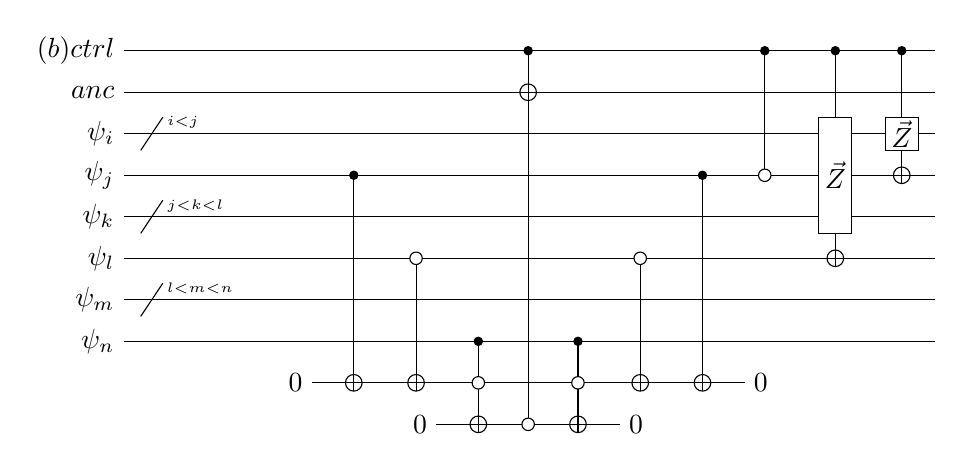
\begin{tikzpicture}[scale=1.000000,x=1pt,y=1pt]
\filldraw[color=white] (0.000000, -7.500000) rectangle (293.000000, 142.500000);
% Drawing wires
% Line 1: c W \text{(b) }ctrl
\draw[color=black] (0.000000,135.000000) -- (293.000000,135.000000);
\draw[color=black] (0.000000,135.000000) node[left] {$\text{(b) }ctrl$};
% Line 2: a W anc
\draw[color=black] (0.000000,120.000000) -- (293.000000,120.000000);
\draw[color=black] (0.000000,120.000000) node[left] {$anc$};
% Line 3: i W \psi_i
\draw[color=black] (0.000000,105.000000) -- (293.000000,105.000000);
\draw[color=black] (0.000000,105.000000) node[left] {$\psi_i$};
% Line 4: j W \psi_j
\draw[color=black] (0.000000,90.000000) -- (293.000000,90.000000);
\draw[color=black] (0.000000,90.000000) node[left] {$\psi_j$};
% Line 5: k W \psi_k
\draw[color=black] (0.000000,75.000000) -- (293.000000,75.000000);
\draw[color=black] (0.000000,75.000000) node[left] {$\psi_k$};
% Line 6: l W \psi_l
\draw[color=black] (0.000000,60.000000) -- (293.000000,60.000000);
\draw[color=black] (0.000000,60.000000) node[left] {$\psi_l$};
% Line 7: m W \psi_m
\draw[color=black] (0.000000,45.000000) -- (293.000000,45.000000);
\draw[color=black] (0.000000,45.000000) node[left] {$\psi_m$};
% Line 8: n W \psi_n
\draw[color=black] (0.000000,30.000000) -- (293.000000,30.000000);
\draw[color=black] (0.000000,30.000000) node[left] {$\psi_n$};
% Line 9: c0 W 0 0
\draw[color=black] (60.500000,15.000000) -- (231.500000,15.000000);
% Line 10: c1 W 0 0
\draw[color=black] (105.500000,0.000000) -- (186.500000,0.000000);
% Done with wires; drawing gates
% Line 12: i / ^{i<j}
\draw (6.000000, 99.000000) -- (14.000000, 111.000000);
\draw (12.000000, 108.000000) node[right] {$\scriptstyle{^{i<j}}$};
% Line 13: k / ^{j<k<l}
\draw (6.000000, 69.000000) -- (14.000000, 81.000000);
\draw (12.000000, 78.000000) node[right] {$\scriptstyle{^{j<k<l}}$};
% Line 14: m / ^{l<m<n}
\draw (6.000000, 39.000000) -- (14.000000, 51.000000);
\draw (12.000000, 48.000000) node[right] {$\scriptstyle{^{l<m<n}}$};
% Line 15: c a i j k l m n c0 c1 LABEL
% Line 16: c0 START
\draw[color=black] (68.000000,15.000000) node[fill=white,left,minimum height=15.000000pt,minimum width=15.000000pt,inner sep=0pt] {\phantom{$0$}};
\draw[color=black] (68.000000,15.000000) node[left] {$0$};
% Line 17: j +c0
\draw (83.000000,90.000000) -- (83.000000,15.000000);
\filldraw (83.000000, 90.000000) circle(1.500000pt);
\begin{scope}
\draw[fill=white] (83.000000, 15.000000) circle(3.000000pt);
\clip (83.000000, 15.000000) circle(3.000000pt);
\draw (80.000000, 15.000000) -- (86.000000, 15.000000);
\draw (83.000000, 12.000000) -- (83.000000, 18.000000);
\end{scope}
% Line 18: -l +c0
\draw (105.500000,60.000000) -- (105.500000,15.000000);
\draw[fill=white] (105.500000, 60.000000) circle(2.250000pt);
\begin{scope}
\draw[fill=white] (105.500000, 15.000000) circle(3.000000pt);
\clip (105.500000, 15.000000) circle(3.000000pt);
\draw (102.500000, 15.000000) -- (108.500000, 15.000000);
\draw (105.500000, 12.000000) -- (105.500000, 18.000000);
\end{scope}
% Line 19: c1 START
\draw[color=black] (113.000000,0.000000) node[fill=white,left,minimum height=15.000000pt,minimum width=15.000000pt,inner sep=0pt] {\phantom{$0$}};
\draw[color=black] (113.000000,0.000000) node[left] {$0$};
% Line 20: n -c0 +c1
\draw (128.000000,30.000000) -- (128.000000,0.000000);
\filldraw (128.000000, 30.000000) circle(1.500000pt);
\draw[fill=white] (128.000000, 15.000000) circle(2.250000pt);
\begin{scope}
\draw[fill=white] (128.000000, 0.000000) circle(3.000000pt);
\clip (128.000000, 0.000000) circle(3.000000pt);
\draw (125.000000, 0.000000) -- (131.000000, 0.000000);
\draw (128.000000, -3.000000) -- (128.000000, 3.000000);
\end{scope}
% Line 21: c -c1 +a
\draw (146.000000,135.000000) -- (146.000000,0.000000);
\filldraw (146.000000, 135.000000) circle(1.500000pt);
\draw[fill=white] (146.000000, 0.000000) circle(2.250000pt);
\begin{scope}
\draw[fill=white] (146.000000, 120.000000) circle(3.000000pt);
\clip (146.000000, 120.000000) circle(3.000000pt);
\draw (143.000000, 120.000000) -- (149.000000, 120.000000);
\draw (146.000000, 117.000000) -- (146.000000, 123.000000);
\end{scope}
% Line 22: n -c0 +c1
\draw (164.000000,30.000000) -- (164.000000,0.000000);
\filldraw (164.000000, 30.000000) circle(1.500000pt);
\draw[fill=white] (164.000000, 15.000000) circle(2.250000pt);
\begin{scope}
\draw[fill=white] (164.000000, 0.000000) circle(3.000000pt);
\clip (164.000000, 0.000000) circle(3.000000pt);
\draw (161.000000, 0.000000) -- (167.000000, 0.000000);
\draw (164.000000, -3.000000) -- (164.000000, 3.000000);
\end{scope}
% Line 23: c1 END
\draw[color=black] (179.000000,0.000000) node[fill=white,right,minimum height=15.000000pt,minimum width=15.000000pt,inner sep=0pt] {\phantom{$0$}};
\draw[color=black] (179.000000,0.000000) node[right] {$0$};
% Line 24: -l +c0
\draw (186.500000,60.000000) -- (186.500000,15.000000);
\draw[fill=white] (186.500000, 60.000000) circle(2.250000pt);
\begin{scope}
\draw[fill=white] (186.500000, 15.000000) circle(3.000000pt);
\clip (186.500000, 15.000000) circle(3.000000pt);
\draw (183.500000, 15.000000) -- (189.500000, 15.000000);
\draw (186.500000, 12.000000) -- (186.500000, 18.000000);
\end{scope}
% Line 25: j +c0
\draw (209.000000,90.000000) -- (209.000000,15.000000);
\filldraw (209.000000, 90.000000) circle(1.500000pt);
\begin{scope}
\draw[fill=white] (209.000000, 15.000000) circle(3.000000pt);
\clip (209.000000, 15.000000) circle(3.000000pt);
\draw (206.000000, 15.000000) -- (212.000000, 15.000000);
\draw (209.000000, 12.000000) -- (209.000000, 18.000000);
\end{scope}
% Line 26: c0 END
\draw[color=black] (224.000000,15.000000) node[fill=white,right,minimum height=15.000000pt,minimum width=15.000000pt,inner sep=0pt] {\phantom{$0$}};
\draw[color=black] (224.000000,15.000000) node[right] {$0$};
% Line 27: c -j
\draw (231.500000,135.000000) -- (231.500000,90.000000);
\filldraw (231.500000, 135.000000) circle(1.500000pt);
\draw[fill=white] (231.500000, 90.000000) circle(2.250000pt);
% Line 29: i j k G $\vec{Z}$ c +l
\draw (257.000000,135.000000) -- (257.000000,60.000000);
\begin{scope}
\draw[fill=white] (257.000000, 90.000000) +(-45.000000:8.485281pt and 29.698485pt) -- +(45.000000:8.485281pt and 29.698485pt) -- +(135.000000:8.485281pt and 29.698485pt) -- +(225.000000:8.485281pt and 29.698485pt) -- cycle;
\clip (257.000000, 90.000000) +(-45.000000:8.485281pt and 29.698485pt) -- +(45.000000:8.485281pt and 29.698485pt) -- +(135.000000:8.485281pt and 29.698485pt) -- +(225.000000:8.485281pt and 29.698485pt) -- cycle;
\draw (257.000000, 90.000000) node {$\vec{Z}$};
\end{scope}
\filldraw (257.000000, 135.000000) circle(1.500000pt);
\begin{scope}
\draw[fill=white] (257.000000, 60.000000) circle(3.000000pt);
\clip (257.000000, 60.000000) circle(3.000000pt);
\draw (254.000000, 60.000000) -- (260.000000, 60.000000);
\draw (257.000000, 57.000000) -- (257.000000, 63.000000);
\end{scope}
% Line 30: i G $\vec{Z}$ c +j
\draw (281.000000,135.000000) -- (281.000000,90.000000);
\begin{scope}
\draw[fill=white] (281.000000, 105.000000) +(-45.000000:8.485281pt and 8.485281pt) -- +(45.000000:8.485281pt and 8.485281pt) -- +(135.000000:8.485281pt and 8.485281pt) -- +(225.000000:8.485281pt and 8.485281pt) -- cycle;
\clip (281.000000, 105.000000) +(-45.000000:8.485281pt and 8.485281pt) -- +(45.000000:8.485281pt and 8.485281pt) -- +(135.000000:8.485281pt and 8.485281pt) -- +(225.000000:8.485281pt and 8.485281pt) -- cycle;
\draw (281.000000, 105.000000) node {$\vec{Z}$};
\end{scope}
\filldraw (281.000000, 135.000000) circle(1.500000pt);
\begin{scope}
\draw[fill=white] (281.000000, 90.000000) circle(3.000000pt);
\clip (281.000000, 90.000000) circle(3.000000pt);
\draw (278.000000, 90.000000) -- (284.000000, 90.000000);
\draw (281.000000, 87.000000) -- (281.000000, 93.000000);
\end{scope}
% Done with gates; drawing ending labels
% Done with ending labels; drawing cut lines and comments
% Done with comments
\end{tikzpicture}
